\section{E-TCP/NC}
\subsection{前向重传机制}
\begin{frame}
	\frametitle{E-TCP/NC头部}
	为了支撑E-TCP/NC的新特性,设计了新的头部。
	\begin{figure}
		\hspace{-1.5em}
		\includegraphics[height=2.8cm]{figures/newheader.eps}
		\caption{新NC头部设计}
		\label{fig:ncheader}
	\end{figure}
	添加了\emph{Pid}和\emph{Pid-reply}。
	\emph{Pid}表示编码报文的编号;
	如果此报文为ACK报文的话,
	\emph{Pid-reply}表示这个ACK报文是由编号为\emph{Pid-reply}的报文激发的。
\end{frame}
%%TCP/NC的突发丢包问题
\begin{frame}
	\frametitle{TCP/NC的突发丢包问题}
	\begin{columns}
		\begin{column}{0.5\textwidth}
			TCP/NC将重传的任务全部交给上层TCP,
			而TCP-Reno无法很好地处理一个RTO内的连续报文丢失。
			在未发生超时重传时,TCP层单个、按序地在多个RTT内重传多个丢失的报文。
		\end{column}
		\begin{column}{0.5\textwidth}
			\begin{figure}
				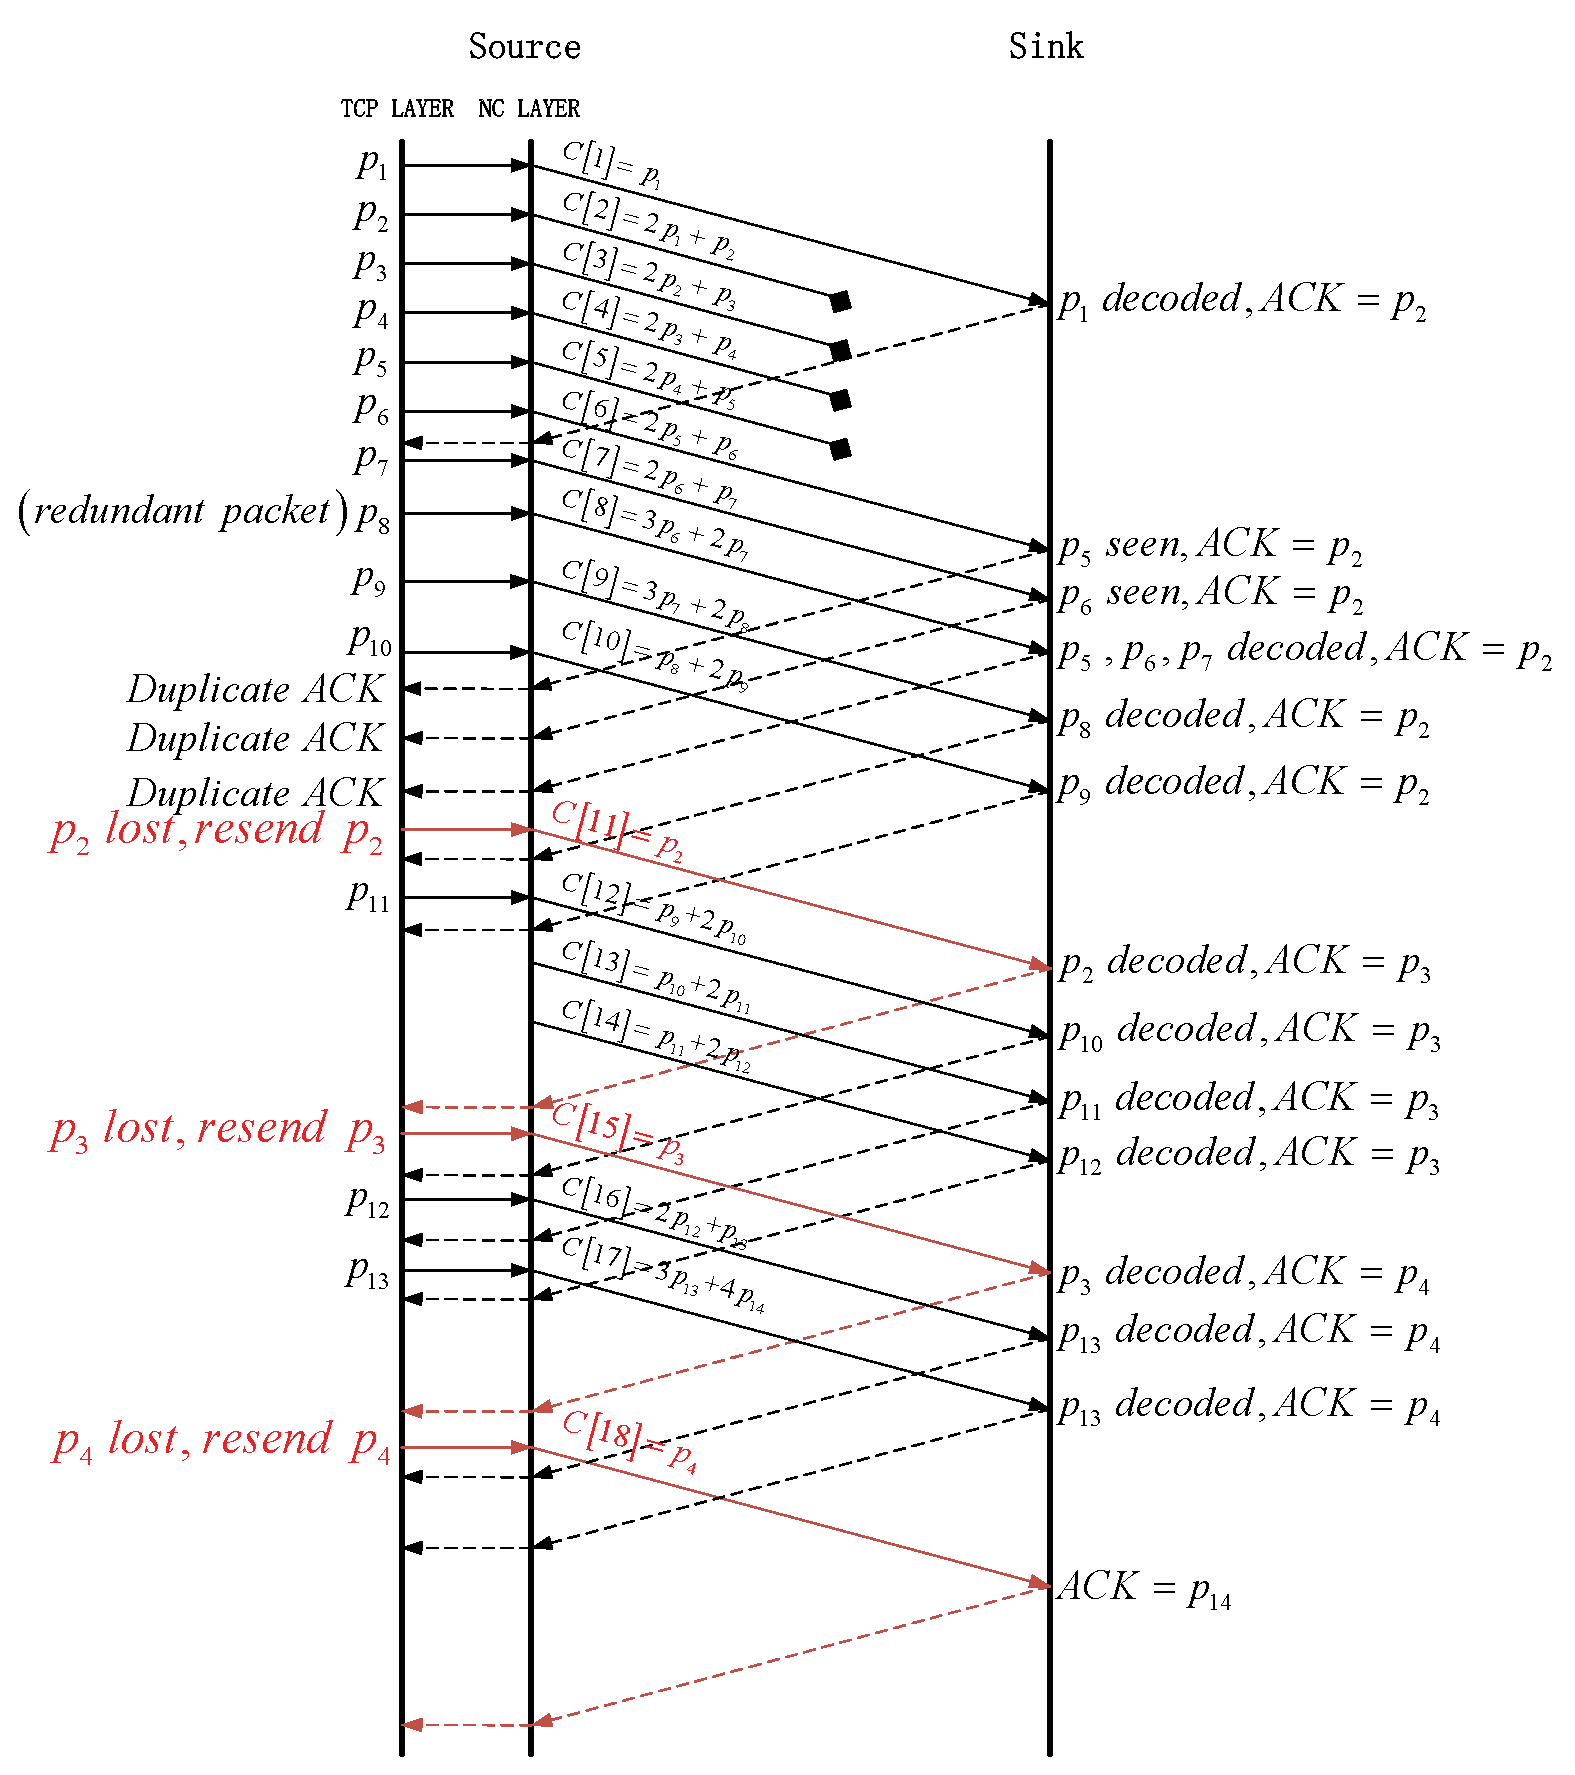
\includegraphics[height=5cm]{../figures/fr.eps}
				\label{原有TCP/NC的重传机制}
			\end{figure}
		\end{column}
	\end{columns}
\end{frame}

%%改进方法
\begin{frame}
	\frametitle{改进方法}
	\begin{columns}
	\begin{column}{0.5\textwidth}
		目标:发送端在一个RTT内重传所有丢失的报文。
		\\
		首先需要定位丢包,确定丢了哪些报文。
	\end{column}
	\hspace{2em}
	\begin{column}{0.5\textwidth}
		\begin{figure}
			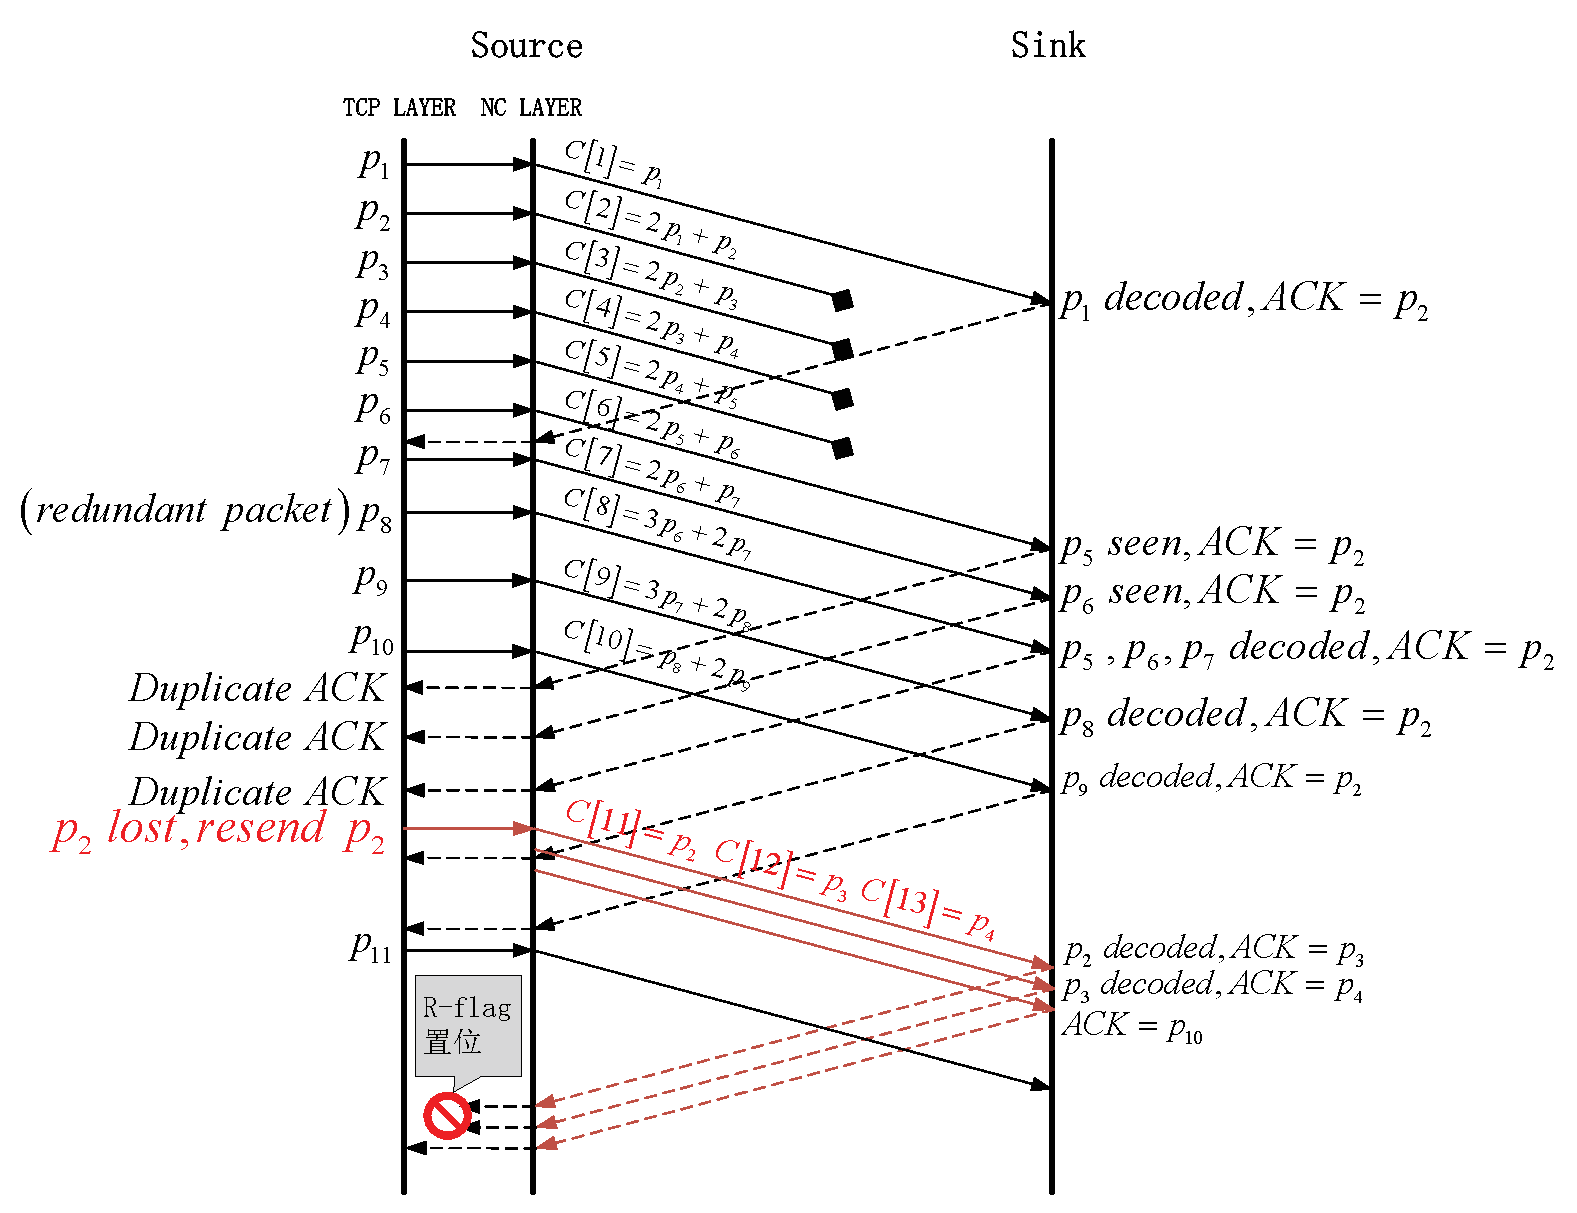
\includegraphics[height=5cm]{../figures/newfr.eps}
			\label{改进重传机制}
		\end{figure}
	\end{column}
	\end{columns}
\end{frame}
\begin{frame}
	\begin{figure}
		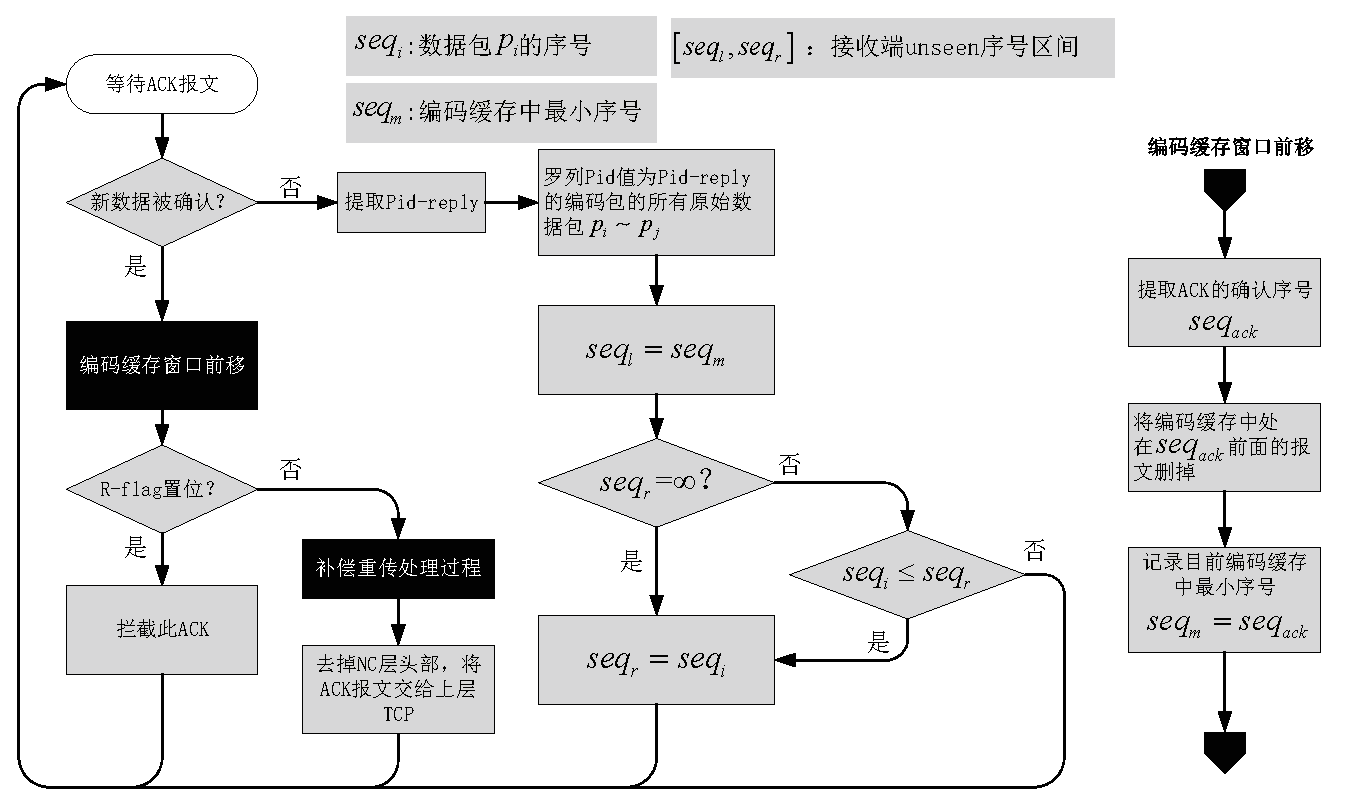
\includegraphics[height=5cm]{../figures/fr-rcvack.eps}
	\end{figure}
\end{frame}



\subsection{自适应冗余}
%%自适应冗余度算法
\begin{frame}
	\frametitle{自适应冗余度算法}
	TCP/NC中冗余度\emph{R}的设置很关键。
	现实中的网络环境,尤其是无线环境,其丢包率是在变动的。
	在设置冗余因子时,如果\emph{R}过小,那么冗余信息不足以掩盖链路中的丢包;如果\emph{R}值过大,编码码率就过小,降低网络的有效吞吐率。
	因此需要找出一种能够根据网络状况自适应调整冗余度的方法,最大化地利用网络带宽。
	\\
	\vspace{1em}
	利用新NC头部的\emph{Pid}和\emph{Pid-reply}字段,
	发送端可以精确知道网络中丢包情况,即丢包率$\rho$。
	\\
	更新冗余度方法如下:
	\begin{equation}
	R=\dfrac{1}{1-\rho}
	\end{equation}
\end{frame}

\subsection{补偿重传}
\frame{
	\frametitle{解码矩阵}
\begin{columns}[onlytextwidth]
	%%\vspace{5em}
	\hspace{-2.0em}
	\begin{column}{0.55\textwidth}
		%%\vspace{-4em}
		\begin{figure}
			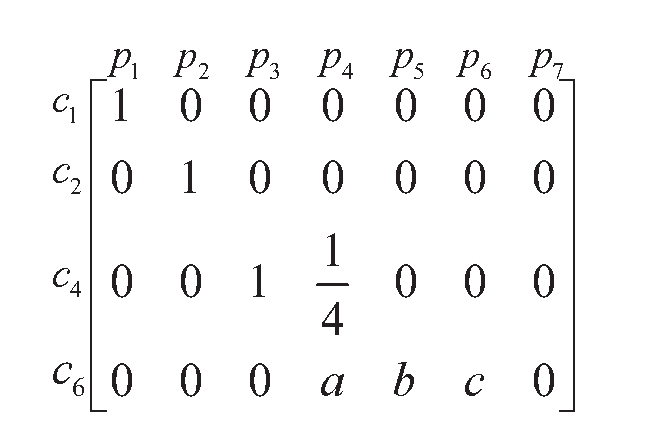
\includegraphics[height=3cm]{figures/matrix.eps}
			\caption{解码矩阵示例}
			\label{fig:jiema}
		\end{figure}
	\end{column}
	\hspace{0.5em}
	\begin{column}{0.55\textwidth}
		\footnotesize
		\begin{block}{解码矩阵}
		图\ref{fig:jiema}表示接收端的解码矩阵的一个示例。
		编码报文$c_3$丢失,$c_4$正确收到,$c_5$又丢失。
		可以看到,接收端可以解码出$p_1$和$p_2$,
		看到(see)$p_3$和$p_4$,
		无法解出$p_3 \sim p_6$。
		\end{block}
	\end{column}
\end{columns}
%\vspace{2em}
以图\ref{fig:jiema}为例,
解码矩阵还需要2个由$p_3$到$p_6$组成的编码包即可解码出$p_3$和$p_6$。
如果能让发送端了解到这个信息,
发送端在下一回合发送过程中,
主动额外地多发相关的编码包,
就可以提前解出$p_3 \sim p_6$,
而无需等到下一次根据冗余度发出的冗余包。
}

%\subsection{反馈重传流程设计}
\frame{
	\frametitle{获码矩阵信息}
	\begin{block}{发送端}
		对于发出去的每个编码包,
		若其编号为\emph{Pid},
		记录编号为\emph{Pid}的编码包由哪几个原始数据包组成,
		以图\ref{fig:codingexp}为例,
		\emph{Pid=1}的编码包由$p_1$、$p_2$、$p_3$和$p_4$组成。
		\\
	\end{block}
	\begin{block}{接收端}
		接收端在发出去的每个ACK报文中都会填写NC头部的\emph{Pid-reply}字段,
		表示此ACK报文是由发送端的编号为\emph{Pid-reply}的编码报文激发的。
	\end{block}
}
%\frame[allowframebreaks]{
\begin{frame}
	\frametitle{获取接收端解码矩阵信息}
	%\vspace{-2em}
	\begin{myDef}[矩阵可解状态]\label{def:kejie}
		假定接收端收到的序号最大的报文为$p_j$,
		已经确认的序号最大的报文为$p_i$。
		如果$i=j$,那么就说接收端解码矩阵为可解状态。
	\end{myDef}
发送端的处理过程如下:
	\begin{block}{步骤}
		%\footnotesize
		\begin{enumerate}[<+-|alert@+>]
			\item 提取\emph{Pid-reply}域,
			罗列值为\emph{Pid-reply}的编码包的所有原始数据包$p_i \sim p_j(i \le j)$;
			\item 如果ACK报文的确认序号$ACK=p_k$,
			那么可知接收端解码矩阵在收到编号为\emph{Pid=Pid-reply}的编码报文时,
			缺失$j-k+1$个编码包才可以变为可解状态;
			%\framebreak

		\end{enumerate}
	\end{block}
%}
\end{frame}


\begin{frame}
		\frametitle{获取接收端解码矩阵信息}
		\begin{block}{步骤( 接上页)}
		\begin{enumerate}[<+-|alert@+>]
	\addtocounter{enumi}{2}
				\item 更新\emph{loss}和\emph{last\_loss}变量,
	其中\emph{loss}表示接收端解码矩阵变为可解状态所需的组合包个数,\emph{last\_loss}表示\emph{loss}上一次的值。
	\item  计算当前时间$T_{now}$和上一次补偿重传的时间$T_{last}$的差值是否超过RTO。
	如果超过,那么重传当前编码缓存窗口的前\emph{loss}个报文;
	如果未超过,比较\emph{loss}的\emph{last\_loss}的值,
	如果$loss \le last\_loss$,那么不进行补偿重传,
	如果$loss > last\_loss$,说明在$T_{last}$到$T_{now}$这段时间又有报文丢失,
	那么就重传编码缓存窗口的前$loss-last\_loss$个报文。
		\end{enumerate}
		\end{block}
\end{frame}

\begin{frame}
	\frametitle{流程图}
	\begin{figure}
		\hspace{-1.5em}
		%\centering
		%%\hspace{-em}
		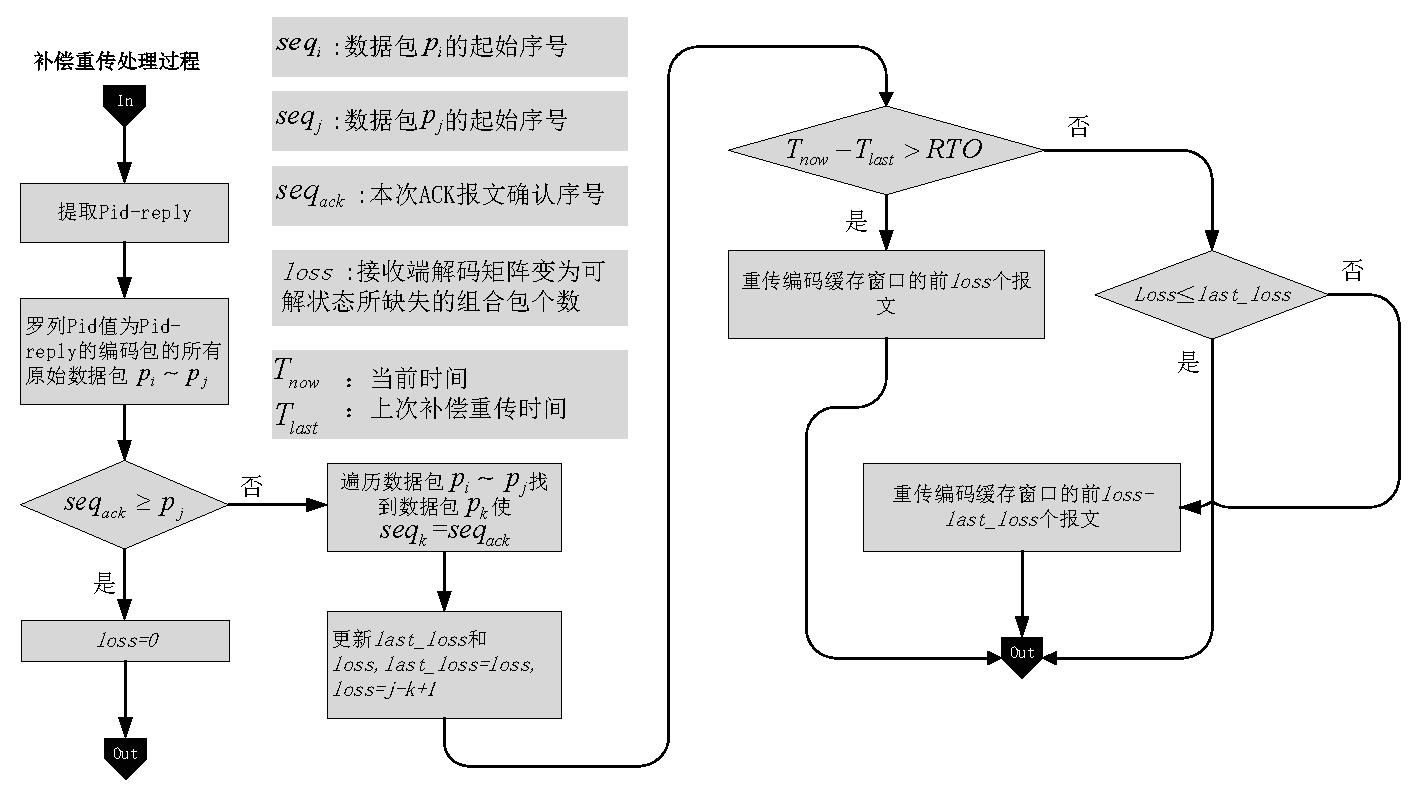
\includegraphics[height=5cm]{../figures/bccc.eps}
		\caption{补偿重传流程图}
		\label{fig:buchang}
	\end{figure}
\end{frame}

\subsection{测试结果和结论}

